\documentclass[margin=0.1in]{standalone}
\usepackage{tikz}
\begin{document}

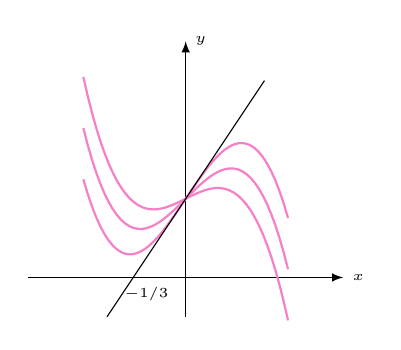
\begin{tikzpicture}[>=latex]
	\draw [->] (-2,0) -- (2,0) node [right] {\tiny \(x\)};
	\draw [->] (0,-0.5) -- (0,3) node [right] {\tiny \(y\)};
	\foreach \n in {1,...,3} \draw [magenta!50, thick , domain=-1.3:1.3, samples = 50] plot(\x , {-pow(\x,3) +0.5*\n*\x+1});
	\draw [thin, domain=-1:1] plot(\x , {1.5*\x+1});
	\node [below] at (-0.5,0) {\tiny \(-1/3\)};
\end{tikzpicture}

\end{document}
